%%%%%%%%%%%%%%%%%%%%%%%%%%%%%%%%%%%%%%%%%%%% DOCUMENT CLASS %%%%%%%%%%%%%%%%%%%%%%%%%%%

\documentclass[12pt]{amsart}
%\documentclass[draft, 12pt]{amsart}


%%%%%%%%%%%%%%%%%%%%%%%%%%%%%%%%%%%%%%%%%%%%%%%%%% STANDARD PACKAGES %%%%%%%%%%%%%%%%%%%%%%%%%%%%%%%%%%%%%%%%%

\usepackage{amssymb,amsmath,amsthm,amscd,mathrsfs,graphicx, color}
\usepackage[cmtip,all,matrix,arrow,tips,curve]{xy}
\usepackage[notref,notcite]{showkeys}
%\usepackage[colorlinks]{hyperref}
\usepackage{multicol}
\usepackage{hyperref}
\usepackage[usenames,dvipsnames]{xcolor}
\hypersetup{colorlinks=true,citecolor=OliveGreen,linkcolor=BrickRed,urlcolor=BlueViolet}
\usepackage[active]{srcltx}
\usepackage{mathpazo}
\usepackage{setspace}\doublespacing 
%Double space, and make it easier for the grader to grade your homework.
%\usepackage{fullpage} 
%Use wide margins, and make it easier for the grader to grade your homework.


%%%%%%%%%%%%%%%%%%%%%%%%%%%%%%%%%%%%%%%%%%%%%% TIKZ FOR GRAPHING %%%%%%%%%%%%%%%%%%%%%%%%%%%%%%%%%%%%%%%%%%%%%%%%%%%%%%%
\usepackage{tikz,pgfplots}


%%%%%%%%%%%%%%%%%%%%%%%%%%%%%%%%%%%%%%%%%%%%%% 		ANSWER BOXES 		%%%%%%%%%%%%%%%%%%%%%%%%%%%%%%%%%%%%%%%%%%%
 \setlength\fboxsep{.3cm}
\setlength\fboxrule{.05cm}

\newcommand*{\boxedcolor}{red}
\makeatletter
\renewcommand{\boxed}[1]{\textcolor{\boxedcolor}{%
  \fbox{\normalcolor\m@th$\displaystyle#1$}}}
\makeatother

\makeatletter
\newcommand{\boxedred}[1]{\textcolor{red}{%
  \fbox{\normalcolor\m@th$\displaystyle#1$}}}
\makeatother

\makeatletter
\newcommand{\boxedblue}[1]{\textcolor{blue}{%
  \fbox{\normalcolor\m@th$\displaystyle#1$}}}
\makeatother




%%%%%%%%%%%%%%%%%%%%%%%%%%%%%%%%%%%%%%%%%%%%%%%%%%%% THEOREM ENVIRONMENTS %%%%%%%%%%%%%%%%%%%%%%%%%%%%%%%%


\numberwithin{equation}{section}
\newtheorem{teo}{Theorem}[section]
\newtheorem{pro}[teo]{Proposition}
\newtheorem{lem}[teo]{Lemma}
\newtheorem{cor}[teo]{Corollary}
\newtheorem{con}[teo]{Conjecture}
\newtheorem{convention}[teo]{}



\newtheorem{teoalpha}{Theorem}
\renewcommand{\theteoalpha}{\Alph{teoalpha}}
\newtheorem{proalpha}[teoalpha]{Proposition}
\newtheorem{coralpha}[teoalpha]{Corollary}


\theoremstyle{definition}
\newtheorem{dfn}[teo]{Definition}
\newtheorem{exa}[teo]{Example}
\newtheorem{que}[teo]{Question}

\theoremstyle{remark}
\newtheorem{rem}[teo]{Remark}
\newtheorem{nte}[teo]{Note}

%%%%%%%%%%%%%%%%%%%%%%%%%%%%%%%%%%%%%%%%%%%%%%% SOME CONDITIONALS FOR NOTES %%%%%%%%%%%%%%%%%%%%%%%%%%%%%%%%%%%

% Declare a new conditional
\newif\ifnotes
\notestrue 	% Show details
%\notesfalse 	% Exclude details


%%%%%%%%%%%%%%%%%%%%%%%%%%%%%%%%%%%%%%%%%%%%% COMMENTS %%%%%%%%%%%%%%%%%%%%%%%%%%%%

\newcommand{\marg}[1]{\normalsize{{\color{red}\footnote{{\color{blue}#1}}}{\marginpar[\vskip -.3cm {\color{BrickRed}\hfill\thefootnote$\implies$}]{\vskip -.3cm{ \color{BrickRed}$\impliedby$\thefootnote}}}}}

\newcommand{\qc}[1]{\marg{#1}}

%%%%%%%%%%%%%%%%%%%%%%%%%%%%%%%%%%%%%%%%%%%%%%%%%%% BEGIN DOCUMENT %%%%%%%%%%%%%%%%%%%%%%%%%%%%%%%%%%%
 
\begin{document}

\bibliographystyle{amsalpha}


%%%%%%%%%%%%%%%%%%%%%%%%%%%%%%%%%%%%%%%%%%%%%%%% AUTHOR INFO %%%%%%%%%%%%%%%%%%%%%%%%%%%%%%%%%%%% 

\author[QI WANG]{QI WANG}
\address{University of Colorado, Department of Mathematics,  Campus Box 395,
Boulder, CO 80309-0395}
\email{casa@math.colorado.edu}
\date{\today}
%\thanks{I would like to take this opportunity to thank my class for their support.}


%%%%%%%%%%%%%%%%%%%%%%%%%%%%%%%%%%%%%%%%%%%%%%%% TITLE AND ABSTRACT %%%%%%%%%%%%%%%%%%%%%%%%%%%%%%%%%%%%

\title[Homework 4]{Homework 4 \\ \ \\  MATH 2001}

\begin{abstract} 
This is the first homework assignment.  The problems are from Hammack \cite[Ch.~2]{H13}:
\begin{itemize}

\item \textbf{Chapter 2}  
\textbf{Section 2.1}, Exercises:  2, 4, 6.
\textbf{Section 2.2}, Exercises:  2, 6.
\textbf{Section 2.3}, Exercises:  8, 10.
\textbf{Section 2.4}, Exercises:  4.



\end{itemize}
\end{abstract}


\maketitle


\tableofcontents

%%%%%%%%%%%%%%%%%%%%%%%%%%%%%%%%%%%%%%%%%%%%%%%% HOMEWORK ASSIGNMENT %%%%%%%%%%%%%%%%%%%%%%%%%%%%%%%%%%%%

%%%%%%%%%%%%%%%%%%%%%%%%%%%%%%%%%%%%%%%%%%%%%%%%%%%%%%%%%%%%%%%%%%%%%%%%%%%%%%%%%%%%%%%%%% CHAPTER 1 %%%%%%%%%%%%%%%%%%%%%%%%%%%%%%%%%%%%%%%%%%%%%%%%%%%%%%%%%%%%%%%%%%%%%%%%%%%%%%%%%%%%%%%%%%%%%%%%%%%


%%%%%%%%%%%%%%%%%%%%%%%%%%%%%%%%%%%%%%%%%%%%%%%% SECTION 1.1 %%%%%%%%%%%%%%%%%%%%%%%%%%%%%%%%%%%%

\section*{Chapter 2 Section 2.1}


%%%%%%%%%%%%%%%%%%%%%%%%%%%%%%%%%%%%%%%%%%%%%%%% EXERCISE 2 %%%%%%%%%%%%%%%%%%%%%%%%%%%%%%%%%%%%

\subsection*{Ch.2, \S 2.1,  Exercise 2}  Decide whether or not the following are statements. In case of a statment, say if it is true or false, if possible: "Every even integer is a real number."


\begin{proof}[Solution to Ch.1, \S 2.1,  Exercise 2] 
\ \\

\begin{center}
It is a statement. \\
It is true.
\end{center}

\end{proof}


%%%%%%%%%%%%%%%%%%%%%%%%%%%%%%%%%%%%%%%%%%%%%%%% EXERCISE 8 %%%%%%%%%%%%%%%%%%%%%%%%%%%%%%%%%%%%


\subsection*{Ch.2, \S 2.1,  Exercise 4}  Decide whether or not the following are statements. In case of a statment, say if it is true or false, if possible: "Set $ \mathbb{Z} $ and set $ \mathbb{N} $"


\begin{proof}[Solution to Ch.1, \S 1.1,  Exercise 8]
\ \\

\begin{center}
It is not a statement.
\end{center}

\end{proof}


%%%%%%%%%%%%%%%%%%%%%%%%%%%%%%%%%%%%%%%%%%%%%%%% EXERCISE 18 %%%%%%%%%%%%%%%%%%%%%%%%%%%%%%%%%%%%


\subsection*{Ch.2, \S 2.1,  Exercise 6}  



\begin{proof}[Solution to Ch.1, \S 2.1,  Exercise 6]
\ \\

\begin{center}
It is a statement. \\
It is true.
\end{center}

\end{proof}


%%%%%%%%%%%%%%%%%%%%%%%%%%%%%%%%%%%%%%%%%%%%%%%% EXERCISE 30 %%%%%%%%%%%%%%%%%%%%%%%%%%%%%%%%%%%%


\subsection*{Ch.1, \S 1.1,  Exercise 30} 


\begin{proof}[Solution to Ch.1, \S 1.1,  Exercise 30]

\end{proof}



%%%%%%%%%%%%%%%%%%%%%%%%%%%%%%%%%%%%%%%%%%%%%%%% EXERCISE 38 %%%%%%%%%%%%%%%%%%%%%%%%%%%%%%%%%%%%


\subsection*{Ch.1, \S 1.1,  Exercise 38} 



\begin{proof}[Solution to Ch.1, \S 1.1,  Exercise 38]

\end{proof}


%%%%%%%%%%%%%%%%%%%%%%%%%%%%%%%%%%%%%%%%%%%%%%%% EXERCISE 40 %%%%%%%%%%%%%%%%%%%%%%%%%%%%%%%%%%%%


\subsection*{Ch.1, \S 1.1,  Exercise 40} 
 Sketch the following set of points in the $x,y$-plane:
$$
S=\{(x,y): x\in [0,1], \ y\in 1,2]\}
$$



\begin{proof}[Solution to Ch.1, \S 1.1,  Exercise 40]
\ 
For this problem I first sketched my own solution by hand.  However, to implement my solution in \LaTeX, I  modifed the tikz code from the webpage: 
\\ 
\url{https://tex.stackexchange.com/questions/140312/tikz-shading-region-bounded-by-several-curves}
\begin{center}
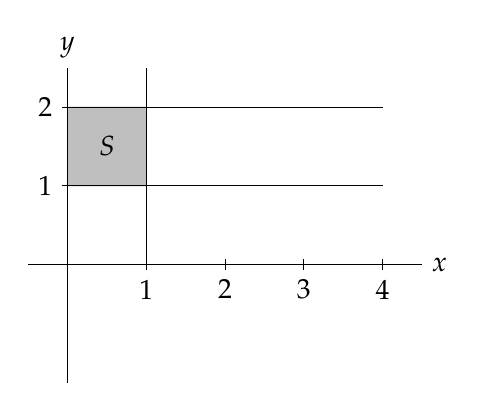
\begin{tikzpicture}
%graph
\draw[draw=gray!50!white,fill=gray!50!white] 
    plot[smooth,samples=100,domain=0:1] (\x,{1}) -- 
    plot[smooth,samples=100,domain=1:0] (\x,{2});
\draw[domain=0:4] plot (\x,{1});
\draw[domain=0:4] plot (\x,{2});
\draw (1,0)--(1,2.5);
%coordinate grid
\draw (-.5,0)--(4.5,0) node[right]{$x$};
\draw (0,-1.5)--(0,2.5) node[above]{$y$};
\foreach \x in {1,2,3,4}
    \draw (\x,2pt)--(\x,-2pt) node[below] {$\x$};
\foreach \y/\ytext in {1,2}
    \draw (2pt,\y)--(-2pt,\y) node[left] {$\y$};    
%labels 
\node at (.5,1.5) {$S$};
\end{tikzpicture}
\end{center}

\end{proof}





\ifnotes


\else
	This is not the full version.  This can be useful if there is scratch work you want to keep for yourself, but you do not want other people to see. 
\fi




\bibliography{templateHW}
\end{document}
